\documentclass[mathserif,t]{beamer}
%\usepackage{Sweave}                                                       
%http://tex.stackexchange.com/questions/105613/footer-in-beamer. Check this out. Frankfurt template.
%http://tex.stackexchange.com/questions/39345/piecewise-highlighting-in-beamer-presentation
%https://joerglenhard.wordpress.com/2011/08/01/beamer-customization-colors/
\usepackage{amssymb,bm,mathtools,amsmath}                                                      
\usepackage{graphicx,caption,float}
\usepackage[UKenglish]{isodate} % for: \today                             
\cleanlookdateon                % for: \today                             

\def\wl{\par\vspace{\baselineskip}\noindent}                             
\def\beginmyfig{\begin{figure}[ht]\begin{center}}                          
\def\endmyfig{\end{center}\end{figure}}                                   

\def\prodl#1#2#3{\prod\limits_{#1=#2}^{#3}}                               
\def\suml#1#2#3{\sum\limits_{#1=#2}^{#3}}                                 
\def\ds{\displaystyle}                                                    
\def\tbf#1{\textbf{#1}}
\def\inv{^{\raisebox{.2ex}{$\scriptscriptstyle-1$}}}
\def\pm{^{\raisebox{.2ex}{$\scriptscriptstyle\prime$}}}
\newcommand{\norm}[1]{\left\lVert#1\right\rVert}
\newcommand{\p}[1]{\left(#1\right)}
\newcommand{\bk}[1]{\left[#1\right]}
\newcommand{\bc}[1]{ \left\{#1\right\} }
\newcommand{\abs}[1]{ \left|#1\right| }
\newcommand{\mat}{ \begin{pmatrix} }
\newcommand{\tam}{ \end{pmatrix} }


% My Beamer Stuff
  \geometry{vmargin=0.3in} % Formating the top bar
  \newcommand{\m}[1]{\mathbf{\bm{#1}}} % Serif bold math

  % My Color Stuff
  \usepackage{xcolor} % http://en.wikibooks.org/wiki/LaTeX/Colors
                      % http://latexcolor.com/
    \definecolor{grey}{rgb}{0.15, 0.15, 0.15} % Sets default color. CHANGE THIS!
    \definecolor{pumpkin}{rgb}{1.0, 0.46, 0.09}
    \definecolor{darktan}{rgb}{1.0, 0.66, 0.07}
    \definecolor{coral}{rgb}{1.0, 0.5, 0.31}
    \definecolor{burlywood}{rgb}{0.98, 0.82 0.6}
    \pagecolor{grey}% Sets the bar color.

  \def\mylitecolor{pumpkin}         % Bullet Color.       CHANGE THIS!
  \def\mycolor{\color{pumpkin}}     % Frame Title Color.  CHANGE THIS!
  \def\mydarkcolor{\color{pumpkin}} % Figure Color.       CHANGE THIS!
    \def\frametitle#1{\vspace{-.32in{\mycolor\textbf{\Large#1}}}}
    \setbeamercolor{itemize item}{fg=\mylitecolor}
    \setbeamercolor{enumerate item}{fg=\mylitecolor}
    \setbeamercolor{itemize subitem}{fg=\mylitecolor}
    \setbeamercolor{itemize subsubitem}{fg=\mylitecolor}
    \setbeamercolor{title}{fg=\mylitecolor}
    \setbeamercolor{footlinecolor}{bg=black!93,fg=\mylitecolor}
    \setbeamercolor{author}{fg=burlywood}
    \setbeamercolor{date}{fg=burlywood}
    \setbeamercolor{institute}{fg=burlywood}

    \usepackage[T1]{fontenc}
    \DeclareCaptionFont{figcol}{\mydarkcolor} %color of the word Figure: in figure captions
    \captionsetup{
      font=scriptsize,
      labelfont={bf,figcol,scriptsize}%,textfont={black}
    }
  \def\hline{ \textcolor{grey}{\hrulefill}\\ }

  % Beamer Footer Stuff:
  %http://tex.stackexchange.com/questions/26476/add-footer-text-to-all-slides-in-beamer
  %http://tex.stackexchange.com/questions/105613/footer-in-beamer
  \beamertemplatenavigationsymbolsempty
  \setbeamertemplate{footline}{
    \hbox{
      \hspace{-.17cm}
      \begin{beamercolorbox}[ht=2mm,dp=8.2mm,leftskip=.3cm,rightskip=.3cm]{footlinecolor}%
        \insertauthor\hfill\insertshorttitle\hfill\insertframenumber/\inserttotalframenumber
      \end{beamercolorbox}
    }
  }

%%%%% Example for embedding images: %%%%%%%%%%%%%%%%%%%%%%%%%%%%%%%%%%%%%%%%%%%%%%%%%%%%%%%%%%%%
%%%\frame{
%%%  \frametitle{How to embed images:}
%%%  \beginmyfig
%%%    \includegraphics[scale=.21]{path/to/file.pdf}
%%%    \caption{Put Caption Here}
%%%  \endmyfig
%%%  \footnote{\tiny \url{https://www.luiarthur.github.com} }
%%%}
% End of Header. Start below beamer below. %%%%%%%%%%%%%%%%%%%%%%%%%%%%%%%%%%%%%%%%%%%%%%%%%%%%%

% defs for this assignment:

\begin{document}
% My Title: {
\def\mytitle{\textbf{Introduction to the Indian Buffet Process}}
  \title[IBP]{\mytitle}
  \author[Arthur Lui]{Arthur Lui}
  \institute{
    AMS\\
    UC Santa Cruz
  }
  {
    \setbeamercolor{background canvas}{bg=grey}
    \frame{\titlepage}
  }
%}

\frame{ %
  \frametitle{Motivation}
  \vspace{15mm}

  Factor Analysis
  \vspace{5mm}
  \begin{itemize}
      \item $\bm{ X = F\Lambda + \epsilon}$, where only $\bm X$ is observed
      \item latent binary feature allocation models
      \item $\bm{ X = ZA + \epsilon}$, where only $\bm X$ is observed
      \item IBP($\alpha$) Prior on $\bm Z$ 
      \item $\bm Z$ is a binary matrix
  \end{itemize}
}

\frame{ %
  \frametitle{Why is it called the Indian Buffet Process?}
  \vspace{5mm}
  
}

\frame{ %
  \frametitle{Traditional Formulation}
  \vspace{5mm}
  
}

\frame{ %
  \frametitle{Stick-breaking Construction}
  \vspace{5mm}

}

\frame{ %
  \frametitle{What does a sample look like?}
  \vspace{5mm}
  \beginmyfig
    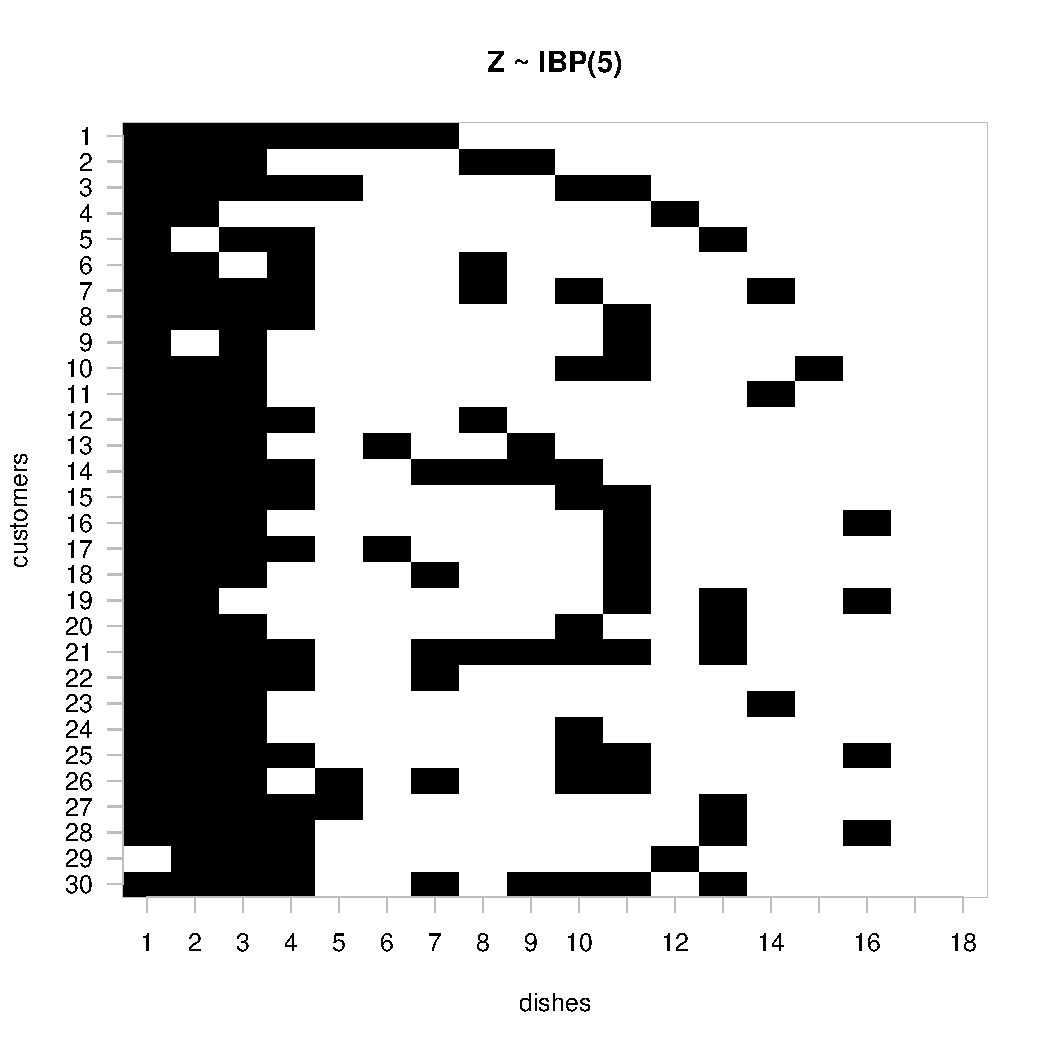
\includegraphics[scale=.4]{../img/Z.pdf}
    \caption{Put Caption Here}
  \endmyfig
}

\frame{ %
  \frametitle{What does a sample look like?}
  \vspace{5mm}
  \beginmyfig
    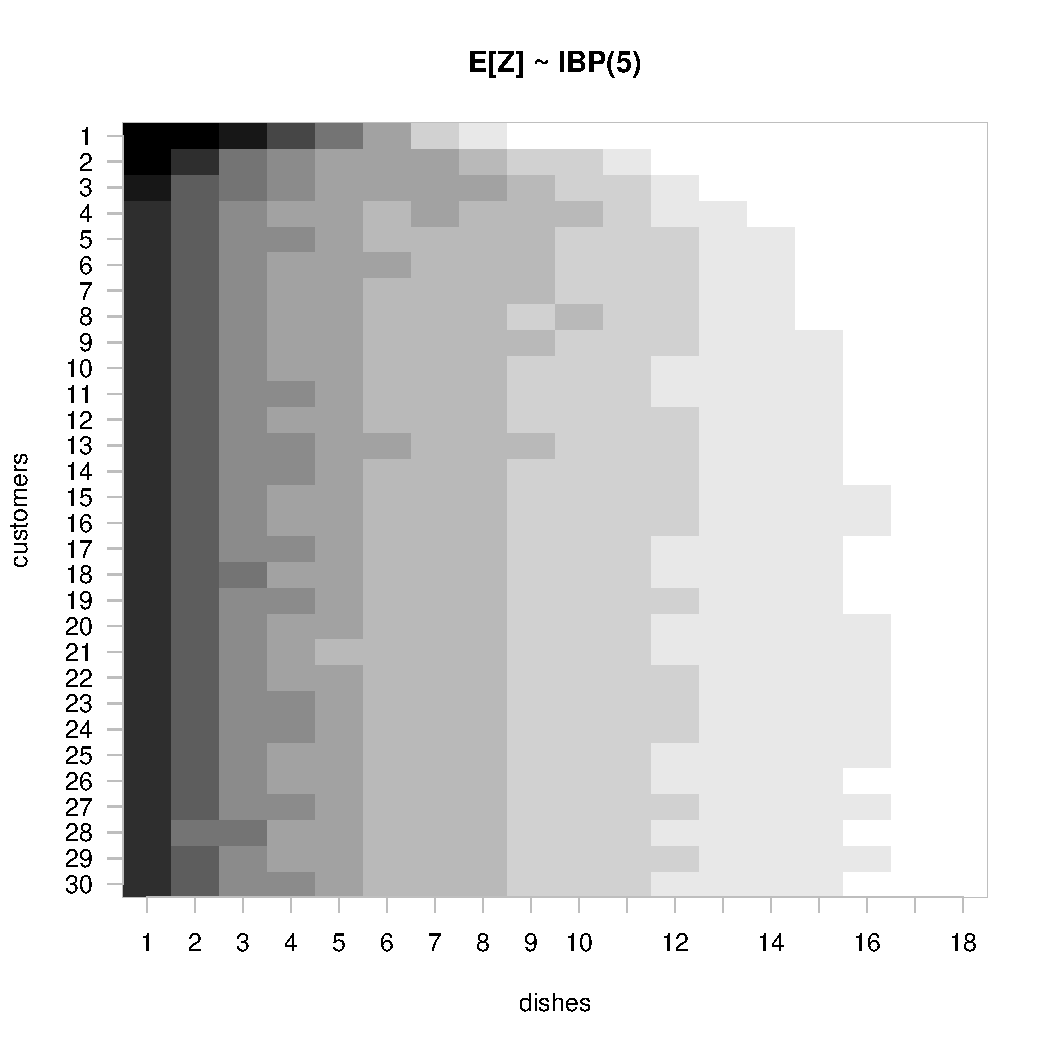
\includegraphics[scale=.4]{../img/EZ.pdf}
    \caption{Put Caption Here}
  \endmyfig
}


\frame{ %
  \frametitle{Toy Example}
  \vspace{5mm}

}

\frame{ %
  \frametitle{Applications}
  \vspace{5mm}

}


\end{document}
% To compile:
%  $ pdflatex *.tex; pdflatex *.tex
